\section{System Model}\label{sec:model}

\subsection{Scenario}
As illustrated in Fig.~\ref{fig:sysmodel}, a LEO satellite (S) equipped with a uniform planar array (UPA) of $N = N_x \times N_y$ antennas transmits navigation/communication signals to $K$ legitimate ground users (GUs) with the aid of a ground-deployed STAR-RIS with $M$ elements.

\begin{figure}[t]
\centering
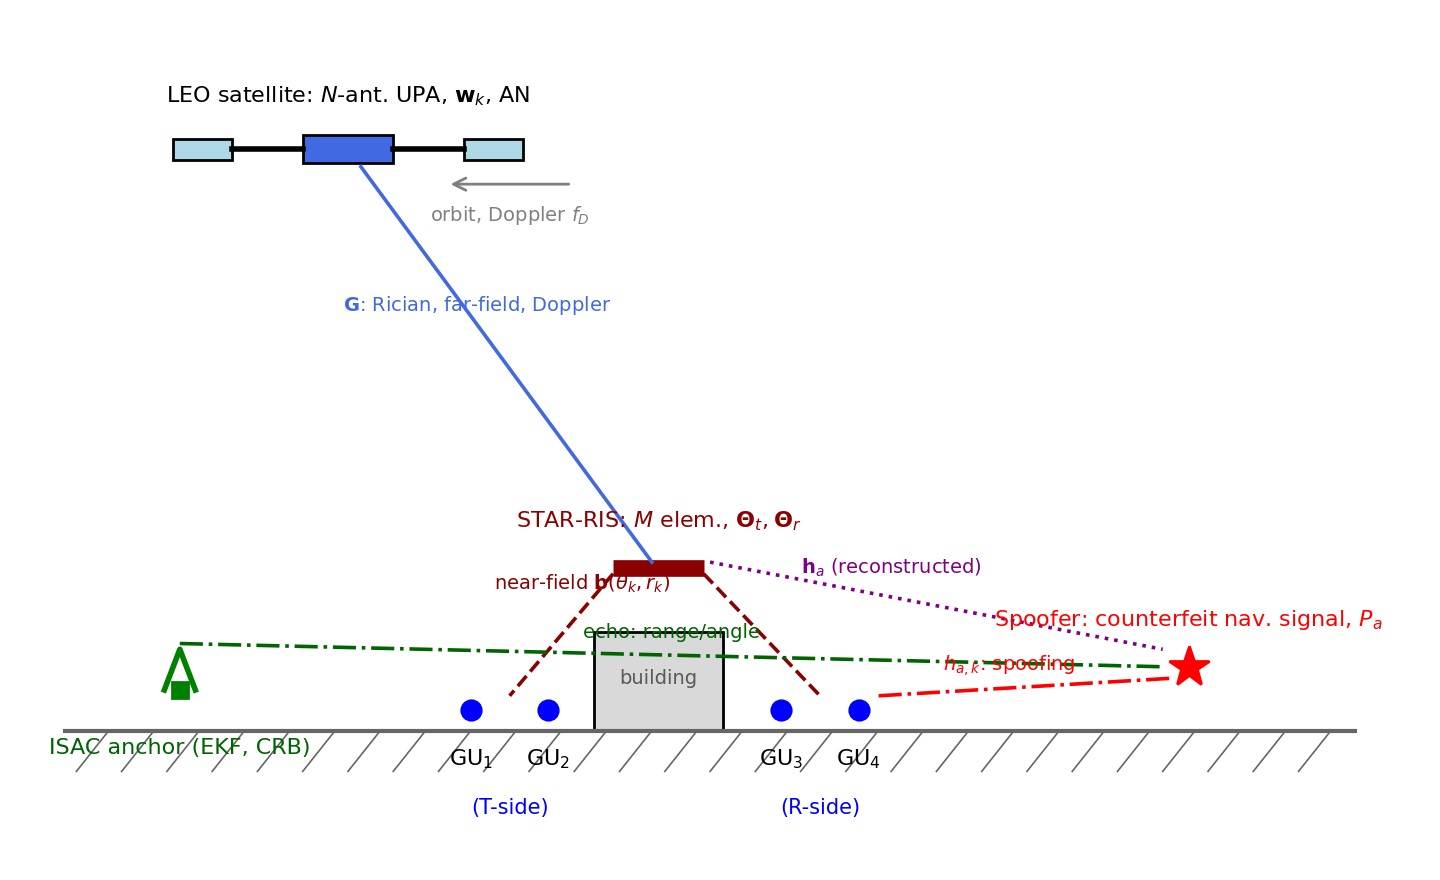
\includegraphics[width=\columnwidth]{figs/fig_system_model.png}
\caption{System model: a LEO satellite serves ground users on both sides of a ground-deployed STAR-RIS; a ground ISAC anchor localizes the active spoofer via near-field echoes.}
\label{fig:sysmodel}
\end{figure} The GUs are partitioned into a transmission-side set $\mathcal{K}_t$ ($|\mathcal{K}_t| = K_t$) and a reflection-side set $\mathcal{K}_r$ ($|\mathcal{K}_r| = K_r$), with $K = K_t + K_r$. An active spoofer (A), located in the reflection half-space, injects a counterfeit navigation signal $s_a(t)$ to mislead the GUs' position estimation. The spoofer is non-cooperative and its channel state information (CSI) is unknown a priori; a ground ISAC anchor node senses the spoofer and provides real-time state estimates (Section~\ref{sec:sensing}).

\subsection{Channel Model}
\subsubsection{Satellite-to-STAR-RIS link (far-field with orbital Doppler)}
Given the large link distance ($\sim$500--1200\,km), the S-to-RIS link is modeled as far-field LoS:
\begin{equation}\label{eq:gsr}
    \mathbf{G} = \sqrt{\beta_{\mathrm{SR}}}\, e^{j 2\pi f_D t} \left( \sqrt{\frac{\kappa}{1+\kappa}}\, \mathbf{a}_M(\vartheta_{\mathrm{SR}})\, \mathbf{a}_N^H(\theta_{\mathrm{SR}}, \phi_{\mathrm{SR}}) + \sqrt{\frac{1}{1+\kappa}}\, \widetilde{\mathbf{G}} \right) \in \mathbb{C}^{M \times N},
\end{equation}
where $\beta_{\mathrm{SR}} = \left(\frac{\lambda}{4\pi d_{\mathrm{SR}}}\right)^2 G_s G_r$ is the large-scale path gain, $f_D$ is the orbital Doppler shift induced by the satellite motion, $\mathbf{a}_N \in \mathbb{C}^{N}$ and $\mathbf{a}_M \in \mathbb{C}^{M}$ are the far-field steering vectors of the satellite array and the STAR-RIS (departure/arrival), $\kappa$ is the Rician factor of the satellite link, and $\widetilde{\mathbf{G}}$ is the scattered (NLoS) component with i.i.d.\ $\mathcal{CN}(0,1)$ entries. The Rician component is essential: a purely LoS rank-one $\mathbf{G}$ would make all cascaded user channels collinear, rendering satellite-side beamforming unable to separate the users.

\subsubsection{STAR-RIS-to-node links (near-field)}
The STAR-RIS aperture is large relative to the RIS-to-user distances, so the GUs and the spoofer lie in its near-field region. The near-field channel vector from the RIS to a node at distance $r$ and angle $\theta$ is
\begin{equation}\label{eq:nfsteer}
    [\mathbf{b}(\theta, r)]_m = \frac{1}{\sqrt{M}} e^{-j\frac{2\pi}{\lambda}(r_m - r)}, \quad r_m = \sqrt{r^2 + \delta_m^2 d^2 - 2 r \delta_m d \sin\theta},
\end{equation}
where $d$ is the element spacing and $\delta_m = \frac{2m - M - 1}{2}$, $m = 1,\dots,M$. Unlike the far-field model, the phase depends on both angle and distance, enabling \emph{distance-angle} resolution.

The overall cascaded channel from the satellite to GU $k \in \mathcal{K}_\chi$, $\chi \in \{t, r\}$, is
\begin{equation}\label{eq:cascade}
    \mathbf{h}_k^H = \sqrt{\beta_k}\, \mathbf{b}^H(\theta_k, r_k)\, \boldsymbol{\Theta}_\chi\, \mathbf{G},
\end{equation}
where $\boldsymbol{\Theta}_t = \mathrm{diag}(\boldsymbol{\theta}_t)$ and $\boldsymbol{\Theta}_r = \mathrm{diag}(\boldsymbol{\theta}_r)$ are the STAR-RIS transmission and reflection coefficient matrices, with $[\boldsymbol{\theta}_\chi]_m = \beta_{\chi,m} e^{j\varphi_{\chi,m}}$, subject to the energy conservation constraint
\begin{equation}\label{eq:unity}
    \beta_{t,m}^2 + \beta_{r,m}^2 = 1, \quad \varphi_{t,m},\varphi_{r,m} \in [0, 2\pi), \ \forall m.
\end{equation}
Similarly, the satellite-to-spoofer cascaded channel is $\mathbf{h}_a^H = \sqrt{\beta_a}\, \mathbf{b}^H(\theta_a, r_a)\, \boldsymbol{\Theta}_r\, \mathbf{G}$.

\subsubsection{Spoofer-to-user link}
The spoofer broadcasts its counterfeit signal to the GUs over channel $h_{a,k} = \sqrt{\beta_{a,k}}\, e^{-j 2\pi \tau_{a,k} f_c}$, where $\tau_{a,k}$ is the propagation delay (the key quantity manipulated in a navigation spoofing attack).

\subsection{Signal Model and Secrecy Rate}
The satellite transmits $\mathbf{x} = \sum_{k=1}^{K} \mathbf{w}_k s_k + \mathbf{z}$, where $\mathbf{w}_k \in \mathbb{C}^N$ is the beamformer for GU $k$, $s_k$ its navigation signal with $\mathbb{E}|s_k|^2 = 1$, and $\mathbf{z} \sim \mathcal{CN}(\mathbf{0}, \mathbf{Z})$ is artificial noise (AN) used for both jamming the spoofer and exciting sensing echoes. The SINR at GU $k$ is
\begin{equation}\label{eq:sinr_u}
    \gamma_k = \frac{|\mathbf{h}_k^H \mathbf{w}_k|^2}{\sum_{j \neq k} |\mathbf{h}_k^H \mathbf{w}_j|^2 + \mathbf{h}_k^H \mathbf{Z} \mathbf{h}_k + P_a |h_{a,k}|^2 + \sigma_k^2},
\end{equation}
where $P_a$ is the spoofer transmit power. The leakage SINR at the spoofer for GU $k$'s signal is
\begin{equation}\label{eq:sinr_a}
    \gamma_{a,k} = \frac{|\mathbf{h}_a^H \mathbf{w}_k|^2}{\sum_{j \neq k} |\mathbf{h}_a^H \mathbf{w}_j|^2 + \mathbf{h}_a^H \mathbf{Z} \mathbf{h}_a + \sigma_a^2}.
\end{equation}
The achievable secrecy rate of GU $k$ against the spoofer is
\begin{equation}\label{eq:secrate}
    R_k^{\mathrm{sec}} = \big[\log_2(1 + \gamma_k) - \log_2(1 + \gamma_{a,k})\big]^+.
\end{equation}

\begin{remark}
Since the spoofer is non-cooperative, $\mathbf{h}_a$ cannot be obtained via pilot-based estimation. Following the sensing-aided paradigm of~\cite{zhao2025nearfield}, $\mathbf{h}_a$ is \emph{reconstructed} from the spoofer's estimated position $(\theta_a, r_a)$ via~\eqref{eq:nfsteer}--\eqref{eq:cascade}.
\end{remark}

\begin{remark}[Why secrecy rate for a spoofing scenario?]
A spoofer is primarily an \emph{injecting} adversary rather than a passive eavesdropper. Our formulation addresses both facets: (i) the spoofing interference $P_a|h_{a,k}|^2$ appears directly in the user SINR~\eqref{eq:sinr_u}, so maximizing the users' rates inherently boosts spoofing resilience; (ii) the secrecy rate~\eqref{eq:secrate} protects the navigation message and its authentication data from being read/relayed by the spoofer (meaconing); (iii) the CRB constraint (Section~\ref{sec:problem}) guarantees that the spoofer itself is accurately localized for subsequent mitigation.
\end{remark}

\subsection{Sensing and Tracking of the Spoofer}\label{sec:sensing}
The ISAC anchor receives echoes of the AN waveform reflected by the spoofer (full-duplex echo reception~\cite{sabharwal2014fullduplex}). Exploiting near-field spherical-wave propagation, the spoofer's 3D velocity is estimated from the variation of the Doppler shift across the spatial domain, and an EKF fuses the predicted and measured states:
\begin{equation}\label{eq:ekf}
    \boldsymbol{\xi}_{a}(t) = [\theta_a, r_a, v_x, v_y, v_z]^T, \qquad \hat{\boldsymbol{\xi}}_{a}(t|t) = \mathrm{EKF}\big(\hat{\boldsymbol{\xi}}_{a}(t|t{-}1),\, \mathbf{y}_{\mathrm{echo}}(t)\big).
\end{equation}
The estimation accuracy is quantified by the CRB of the spoofer parameters $\boldsymbol{\eta} = [\theta_a, r_a]^T$. Given the echo model $\mathbf{y} = \sqrt{P_s}\,\mathbf{b}(\theta_a, r_a) + \mathbf{n}$ with $\mathbf{n} \sim \mathcal{CN}(\mathbf{0}, \sigma^2 \mathbf{I}_M)$ at the anchor, the Fisher information matrix (FIM) is
\begin{equation}\label{eq:fim}
    \mathbf{F} = \frac{2 P_s}{\sigma^2}\, \mathrm{Re}\!\left\{ \mathbf{D}^H \mathbf{D} \right\}, \qquad \mathbf{D} = \left[ \frac{\partial \mathbf{b}}{\partial \theta_a},\ \frac{\partial \mathbf{b}}{\partial r_a} \right],
\end{equation}
and the range CRB is $\mathrm{CRB}_r = [\mathbf{F}^{-1}]_{22}$. Under the far-field approximation, $\partial \mathbf{b}/\partial r_a = \mathbf{0}$, so $\mathbf{F}$ is singular and the range is unobservable --- the key motivation for near-field sensing (cf.\ Section~\ref{sec:results}). The impact of the STAR-RIS phase profile on~\eqref{eq:fim} over the cascaded channel is left to the journal extension.

\subsection{LEO-Specific Considerations}
Compared to the terrestrial baseline~\cite{zhao2025nearfield}, the LEO scenario introduces: (i) time-varying elevation angle and strong orbital Doppler $f_D(t)$ (up to tens of kHz at L/S band), requiring Doppler pre-compensation in~\eqref{eq:gsr}; (ii) large-scale free-space path loss, making the STAR-RIS gain essential; (iii) visibility windows, within which the optimization in Section~\ref{sec:problem} is re-solved per time slot.
